\section{Reasoning Framework Overview\label{sec:framework}}

The design goals of our framework are modularity for the
transformation steps and flexibility with respect to the
underlying inference engine. The modularity allows to reuse
transformation functionality across different WSML variants and
reduces the effort for accomplishing other reasoning tasks. By
reducing WSML to simple Datalog constructs and providing a
respective object model we have reduced the effort of integrating
new reasoners to a minimum\footnote{In fact, the adaptation of the
framework to the MINS rule engine took less then a day.}.

\subsection{Architecture and Internal Layering}
Figure~\ref{fig:layering} shows the basic components of the system
\sgr{it is not clear what "the system" is here.} as well as the
data flow during a prototypical usage scenario. The inner box
shows the currently implemented transformations that are bundled
to reduce the incoming WSML ontology to a Datalog program.
Different implementations of the ReasonerFacade provide the
translation of the generic Datalog program into tool specific
versions.

Queries in fact use the same infrastructure, except that a new transformation pipeline is
composed where the axiomatization and constraint replacement transformations are not included.

{\bf HL: please correct the graphic, meta level axioms are injected
on the wsml level and not on the lower level!

GN: I do not agree, meta level axioms are added in the WSML2Datalog transformer, check the Java code. So the graphics seems to be OK.}

\begin{figure}[h]
    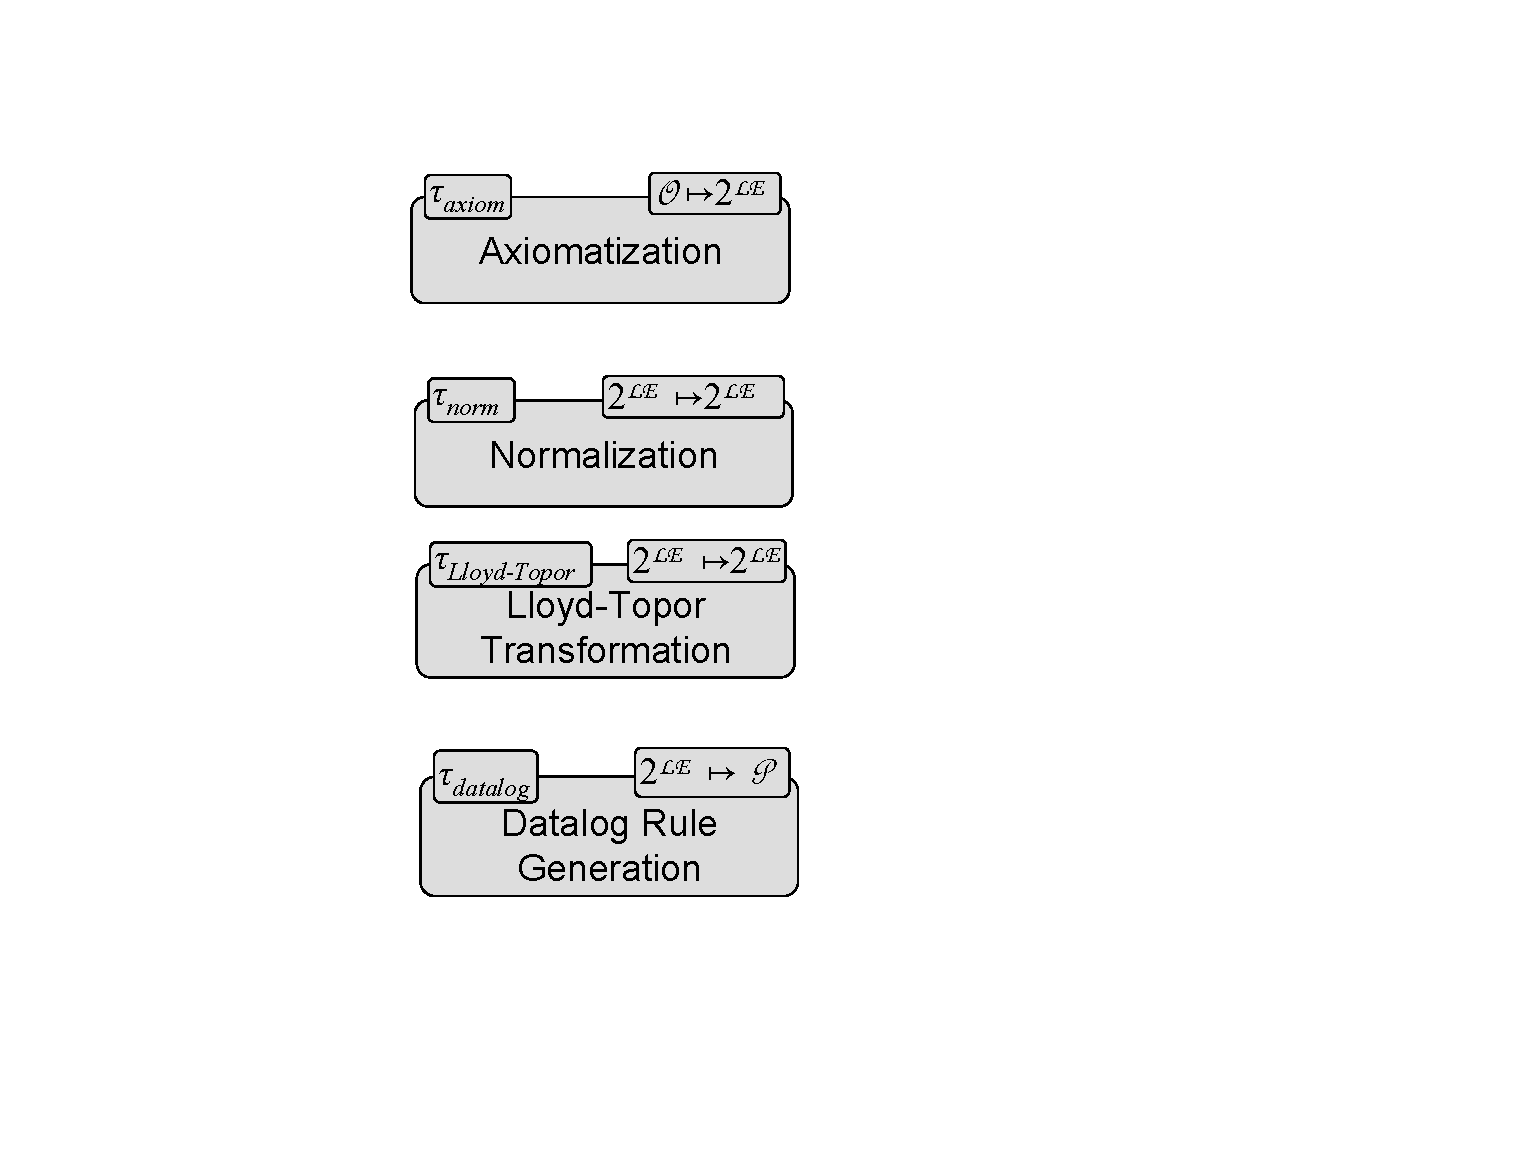
\includegraphics[width=11cm]{figures/layering}
    \centering
    \caption{Layering of the Internal Architecture. \label{fig:layering}}
\end{figure}


\subsection{Interface and Integration with Existing Technology}
So far we have not detailed on what data structure the framework
operates on. One could implement it directly with a parser and
compiler framework that generates some abstract syntax tree for WSML
which is directly transformed to the target format (Datalog).
Although this would have performance advantages, it would greatly
reduce reusability and would make maintenance harder. Our framework is
based on an intermediate object model of the language that is
provided by the WSMO4J\footnote{http://wsmo4j.sourceforge.net}
project. WSMO4J performs the task of parsing and validating WSML ontologies and provides the source object model for our translations. In order to enable the usage of different Datalog
engines we additionally implemented a simple object model for
Datalog that is independent from any particular
engine.

The main Datalog engine we used during our work was the KAON2
inference engine\footnote{KAON2 is available for download from
\url{http://kaon2.semanticweb.org}} \cite{hustadt04reducing}. As we have seen in Section~\ref{sec:datatype_reasoning}, datatype reasoning poses the biggest challenge for the Datalog implementation.
KAON2 provides a very flexible type system that allows for
user-defined datatypes, together with user-defined predicates on
these datatypes, including type checking predicates. Therefore,
KAON2 meets the identified requirements easily. As a matter of
fact, KAON2 already provided most of the required datatypes and
predicates out of the box.

{\bf GN: Perhaps we should include something about MINS?}
